\documentclass{article}
\usepackage[utf8]{inputenc}
\usepackage{graphicx,amsmath,amsfonts,amssymb,caption,subcaption}

\begin{document}
\title{SVVR Assignment 2}
\author{Sander Nugteren (6042023) \and Merel de Groot (6103677)}
\renewcommand{\today}{November 17, 2014}
\maketitle

\section{Visualization Pipeline}
The assignment is to create a visualization pipeline with VTK. The source will be a dataset consisting of images from a CT scanner. These 2D images combined form a 3D image of a body. Using VTK we will create a pipeline that takes the dataset as input and creates a 3D visualization of the body. The order of the sections will correspond to the steps of the pipeline.

\subsection{Source}
The data consists of 94 images created by a CT scanner. Each file is 131,072 bytes and the images are 256x256 or 512x512 pixels in size. Since 131,072 devided by 512x512 is only a half, we know that this is not possible. Deviding 131,072 by 256x256 however, gives us 2 bytes, which is a reasonable size of data per pixel. The collection of binary images is read by using \textsc{VTKImageReader2}.

By default voxels are isotropic, but this has to be adjusted to get a proper view of the head. In this case the voxels need to be adjusted to $(1,1,2)$ to make the data spacing more accurate.

\subsection{Filter: Contour}
At this stage a contour filter is used to create the isosurface. The range of the values is $\left[ 0,  65535.0) \right]$. The suggestion to start with a halfway value only renders a jaw, i.e. the dense bone. But by lowering the value softer tissues become visible. Around $700$ the skin is smooth, showing the soft tissue of the body and when increased to $1200$ we can see the bones. So the isosurfaces correspond to the density of the material.

\subsection{Colours}
Unfortunately VTK maintains a default of a dark blue object on a black background. To make the image more visible, three ways of changing this are implemented:
\begin{itemize}
\item Tell the contour filter stage to not compute scalar values and then set a
	colour in the actor.
\item Tell the mapper stage to ignore scalar values and then set a colour in
	the actor.
\item Tell the mapper what the actual scalar range is.
\end{itemize}
We ended up using the third way to produce our visualisations.

\subsection{Renderer: Setting the Scene}
The renderer configures the visualization in the window. 

There are two models in VTK to manipulate the camera:
\begin{itemize}
\item Camera is focused at a focal point and moves around this focal point using the Elevation, Roll and Azimuth methods.
\item The movement of the camera is centered at the position of the camera and the orientation of the camera is controlled using the Yaw, Roll and Pitch methods.
\end{itemize}


\section{Results}

In figure \ref{fig:skulls} we see two isosurfaces displayed. The head is displayed
from two angles, so that we can see both surfaces in figure \ref{fig:skull1}.
In figure \ref{fig:skull0} we see a tiny scar.
In figure \ref{fig:skull1} we see that behind this scar a tiny blue object is
lodged inside the skull. This might be what killed our victim.
For clarity's sake, we displayed the blue parts without the skin in figure
\ref{fig:jaw}.

\begin{figure}
	\centering
	\begin{subfigure}[b]{0.3\textwidth}
		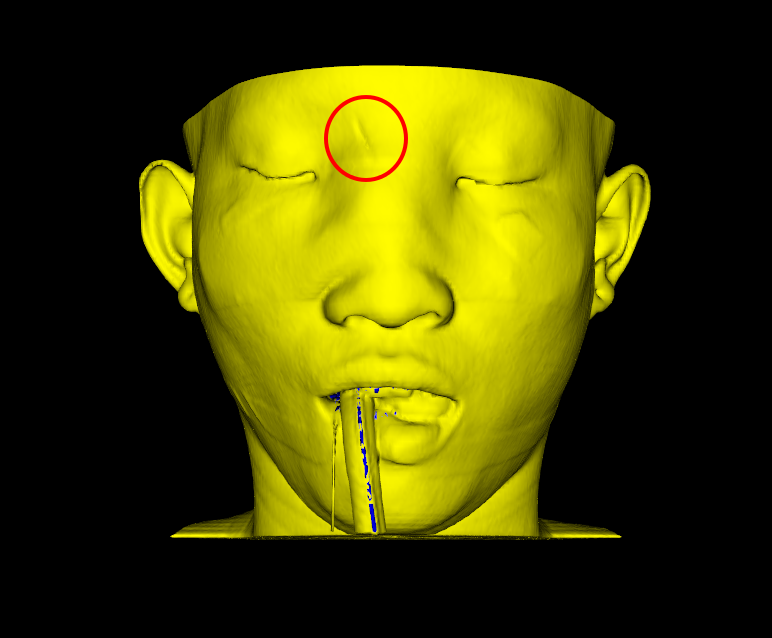
\includegraphics[width=\textwidth]{skull0}
			\caption{Frontal picture of the head. Notice the scar circled in
			red.}
			\label{fig:skull0}
	\end{subfigure}
	\quad
	\begin{subfigure}[b]{0.3\textwidth}
		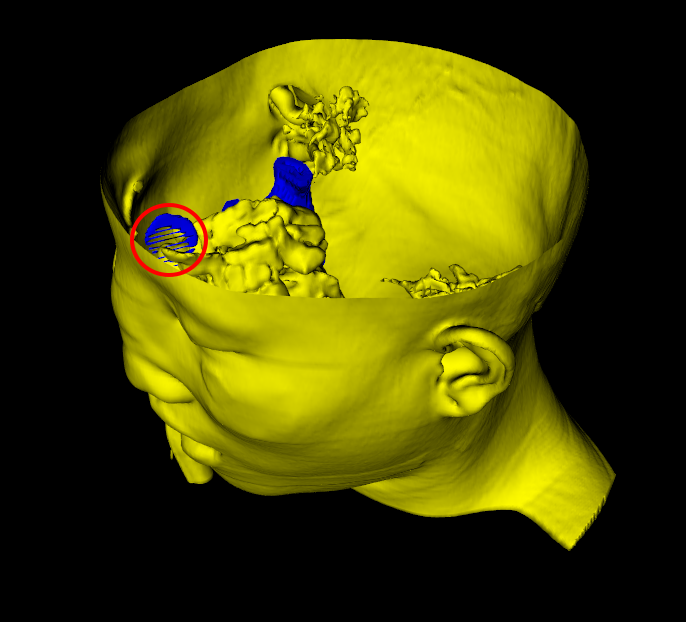
\includegraphics[width=\textwidth]{skull1}
			\caption{Foreign object lodged into head at scar position.}
			\label{fig:skull1}
	\end{subfigure}
	\quad
	\begin{subfigure}[b]{0.3\textwidth}
		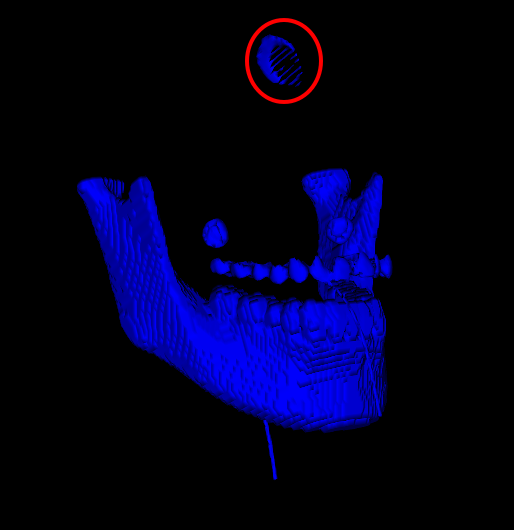
\includegraphics[width=\textwidth]{jaw}
			\caption{Jaw and foreign object only.}
			\label{fig:jaw}
	\end{subfigure}
	\caption{Skin is displayed in yellow (isosurface of 700), dense bones and
	foreign object displayed in blue (isosurface of 3000)}\label{fig:skulls}
\end{figure}

\end{document}
